\documentclass[xcolor=dvipsnames,hyperref={pdfpagelabels=false}]{beamer}

\usetheme{AnnArbor}

\let\Tiny=\tiny

\newcommand{\bi}{\begin{itemize}}
\newcommand{\ei}{\end{itemize}}
\newcommand{\be}{\begin{enumerate}}
\newcommand{\ee}{\end{enumerate}}
\newcommand{\bc}{\begin{center}}
\newcommand{\ec}{\end{center}}
\newcommand{\bd}{\begin{description}}
\newcommand{\ed}{\end{description}}
\newcommand{\I}{\item}
\newcommand{\f}{\frame}
\newcommand{\ft}{\frametitle}

\title{Offline Software Progress}
\subtitle{GlueX Collaboration Meeting}
\author[Mark Ito]{Mark M.\ Ito}
\date{October 4, 2012}
\institute[JLab]{Jefferson Lab}

\begin{document}

\f{\titlepage}

\section{Offline Topics}

\f{
\ft{Code Integrity}
\bi
\I David has looked at two products:
    \bi
    \I scan-build analyzer
    \I cppcheck
    \ei
\I finds things like
    \bi
    \I unused variables
    \I bad free (free'ing somthing not malloc'ed)
    \I various null pointer scenarios
    \I memory leaks
    \ei
\I detailed reports generated, ``explanations'' given
\I downside: most ``bugs'' actually innocuous (false positives)
\ei
}

\f{
\ft{REST Format}

\bi
\I new HDDM (effective) mark-up language for reconstructed data
\I captures data in DANA objects, writes them out
\I can be read in and DANA objects reconstituted
\I large factor of compression over raw MC data
\ei
\bc \bf Related Issues\ec
\bi
\I raw MC event size
    \bi
    \I size of raw events studied
    \I need to account for truth information separately
    \ei
\I proposal for separating truth from fiction
\ei
}

\f{
\ft{Odds and Sods}

\bi
\I Xerces-c 3 support
\I Bourne shell environment set-up is out there now
\I BCAL smearing
\I EVIO-to-DANA conversion
\I Tracking progress
\I Kinematic fitting
\I Analysis tools
\I CCDB
\I 12 GeV Offline Software Review
\ei

}

\section{Data Challenge}

\f{
\ft{Organization}

\bi
\I Wiki page for collecting ideas
\I Bi-weekly data challenge meetings
\I Discussion of analysis tools at bi-weekly Physics Working Group meetings
\ei

\centerline{\bf Decisions/Observations}
\bi
\I need robust SRM
\I JLab farm and on grid
\I huge sample of Pythia data
\I December or January goal for full-scale
\ei

}

\f{
\ft{Mini Data Challenges}

\bi
\I Purpose: develop system for automating large-scale production processing.
    \bi
    \I how to generate and run thousands of jobs
    \I assess their status (before, during, and after they run)
    \I manage all output files and diagnostic data
    \ei
\I With system in place, iteration easy
\I Can then refine:
    \bi
    \I code correctness
    \I execution speed
    \I design and implementation of analysis system
    \I develop goals for full-scale challenge
    \I find bottle-necks at intermediate scale 
    \ei
\ei
}

\f{
\ft{Current Mini-DC Configuration}

\be
\I bggen
    \bi
    \I create 400 k events per job with bggen = 20 s of data
    \I run mcsmear on hdgeant output
    \I write results to tape library
    \I about 7 hours of CPU time
    \I output file is about 14 GB (35 kB per event) 
    \ei
\I hd\_root
    \bi
    \I get bggen data file from library
    \I run reconstruction using hd\_root
    \I write resulting REST file to tape library
    \ei
\ee

}

\f{

\begin{columns}
\column{.35\textwidth}

\bi
\I Perl script and MySQL database: no by-hand operations
\I Output for both written to new tape volume set: /mss/halld/halld-scratch
\I Unit of challenge: 1000 jobs = 5.6 hours of data (1 s = 20 k events)
\ei

\column{.65\textwidth}

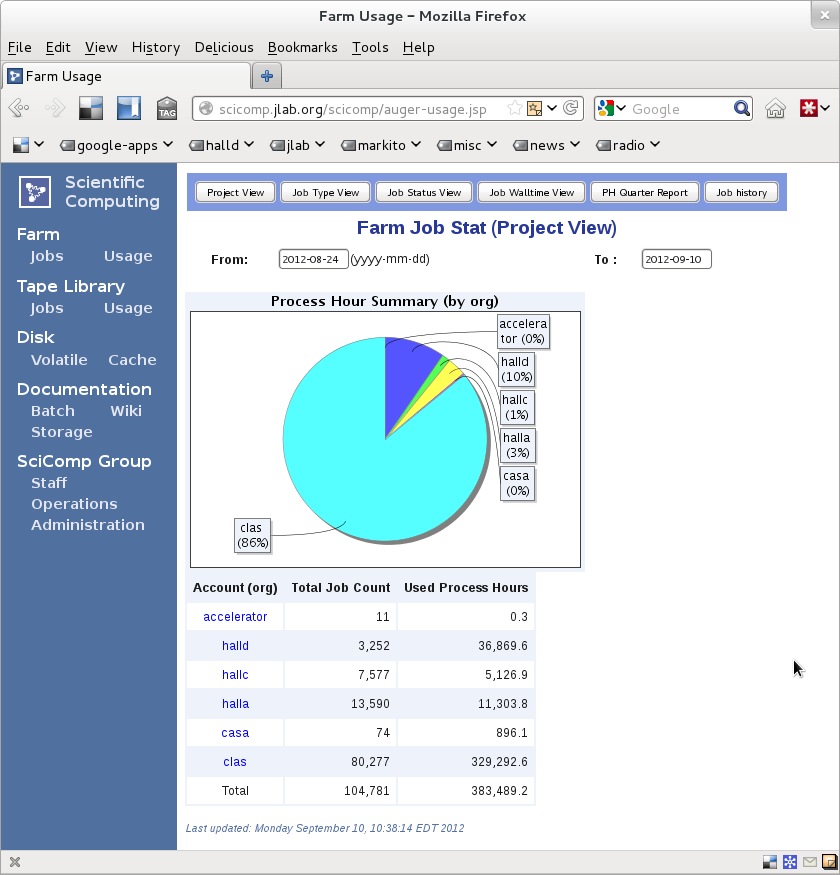
\includegraphics[width=3in]{Farm_usage_2012-09-10.png}

\end{columns}
}

\section{Summary/Conclusions}

\f{
\ft{Summary and Conclusions}

\bi
\I Settled on a compact format for reconstructed data
\I Responding to review recommendations
\I Studying tools for QA of our code
\I Data Challenge technology developing
\I Have the attention of the Computer Center
\I And if there is time...some other items...
\ei
}

\section{JLab Computing Items}

\f{
\ft{GEANT4 Tutorial Workshop}

\begin{columns}
\column{0.5\textwidth}
\bi
\I Held at JLab July 9-13
\I Reprise of 2006 workshop
\I Over 100 participants
\I Many hands-on sessions
\I All talks and tutorials available at http://geant4.slac.stanford.edu/\\
JLAB2012/Agenda.html
\ei
\column{0.5\textwidth}
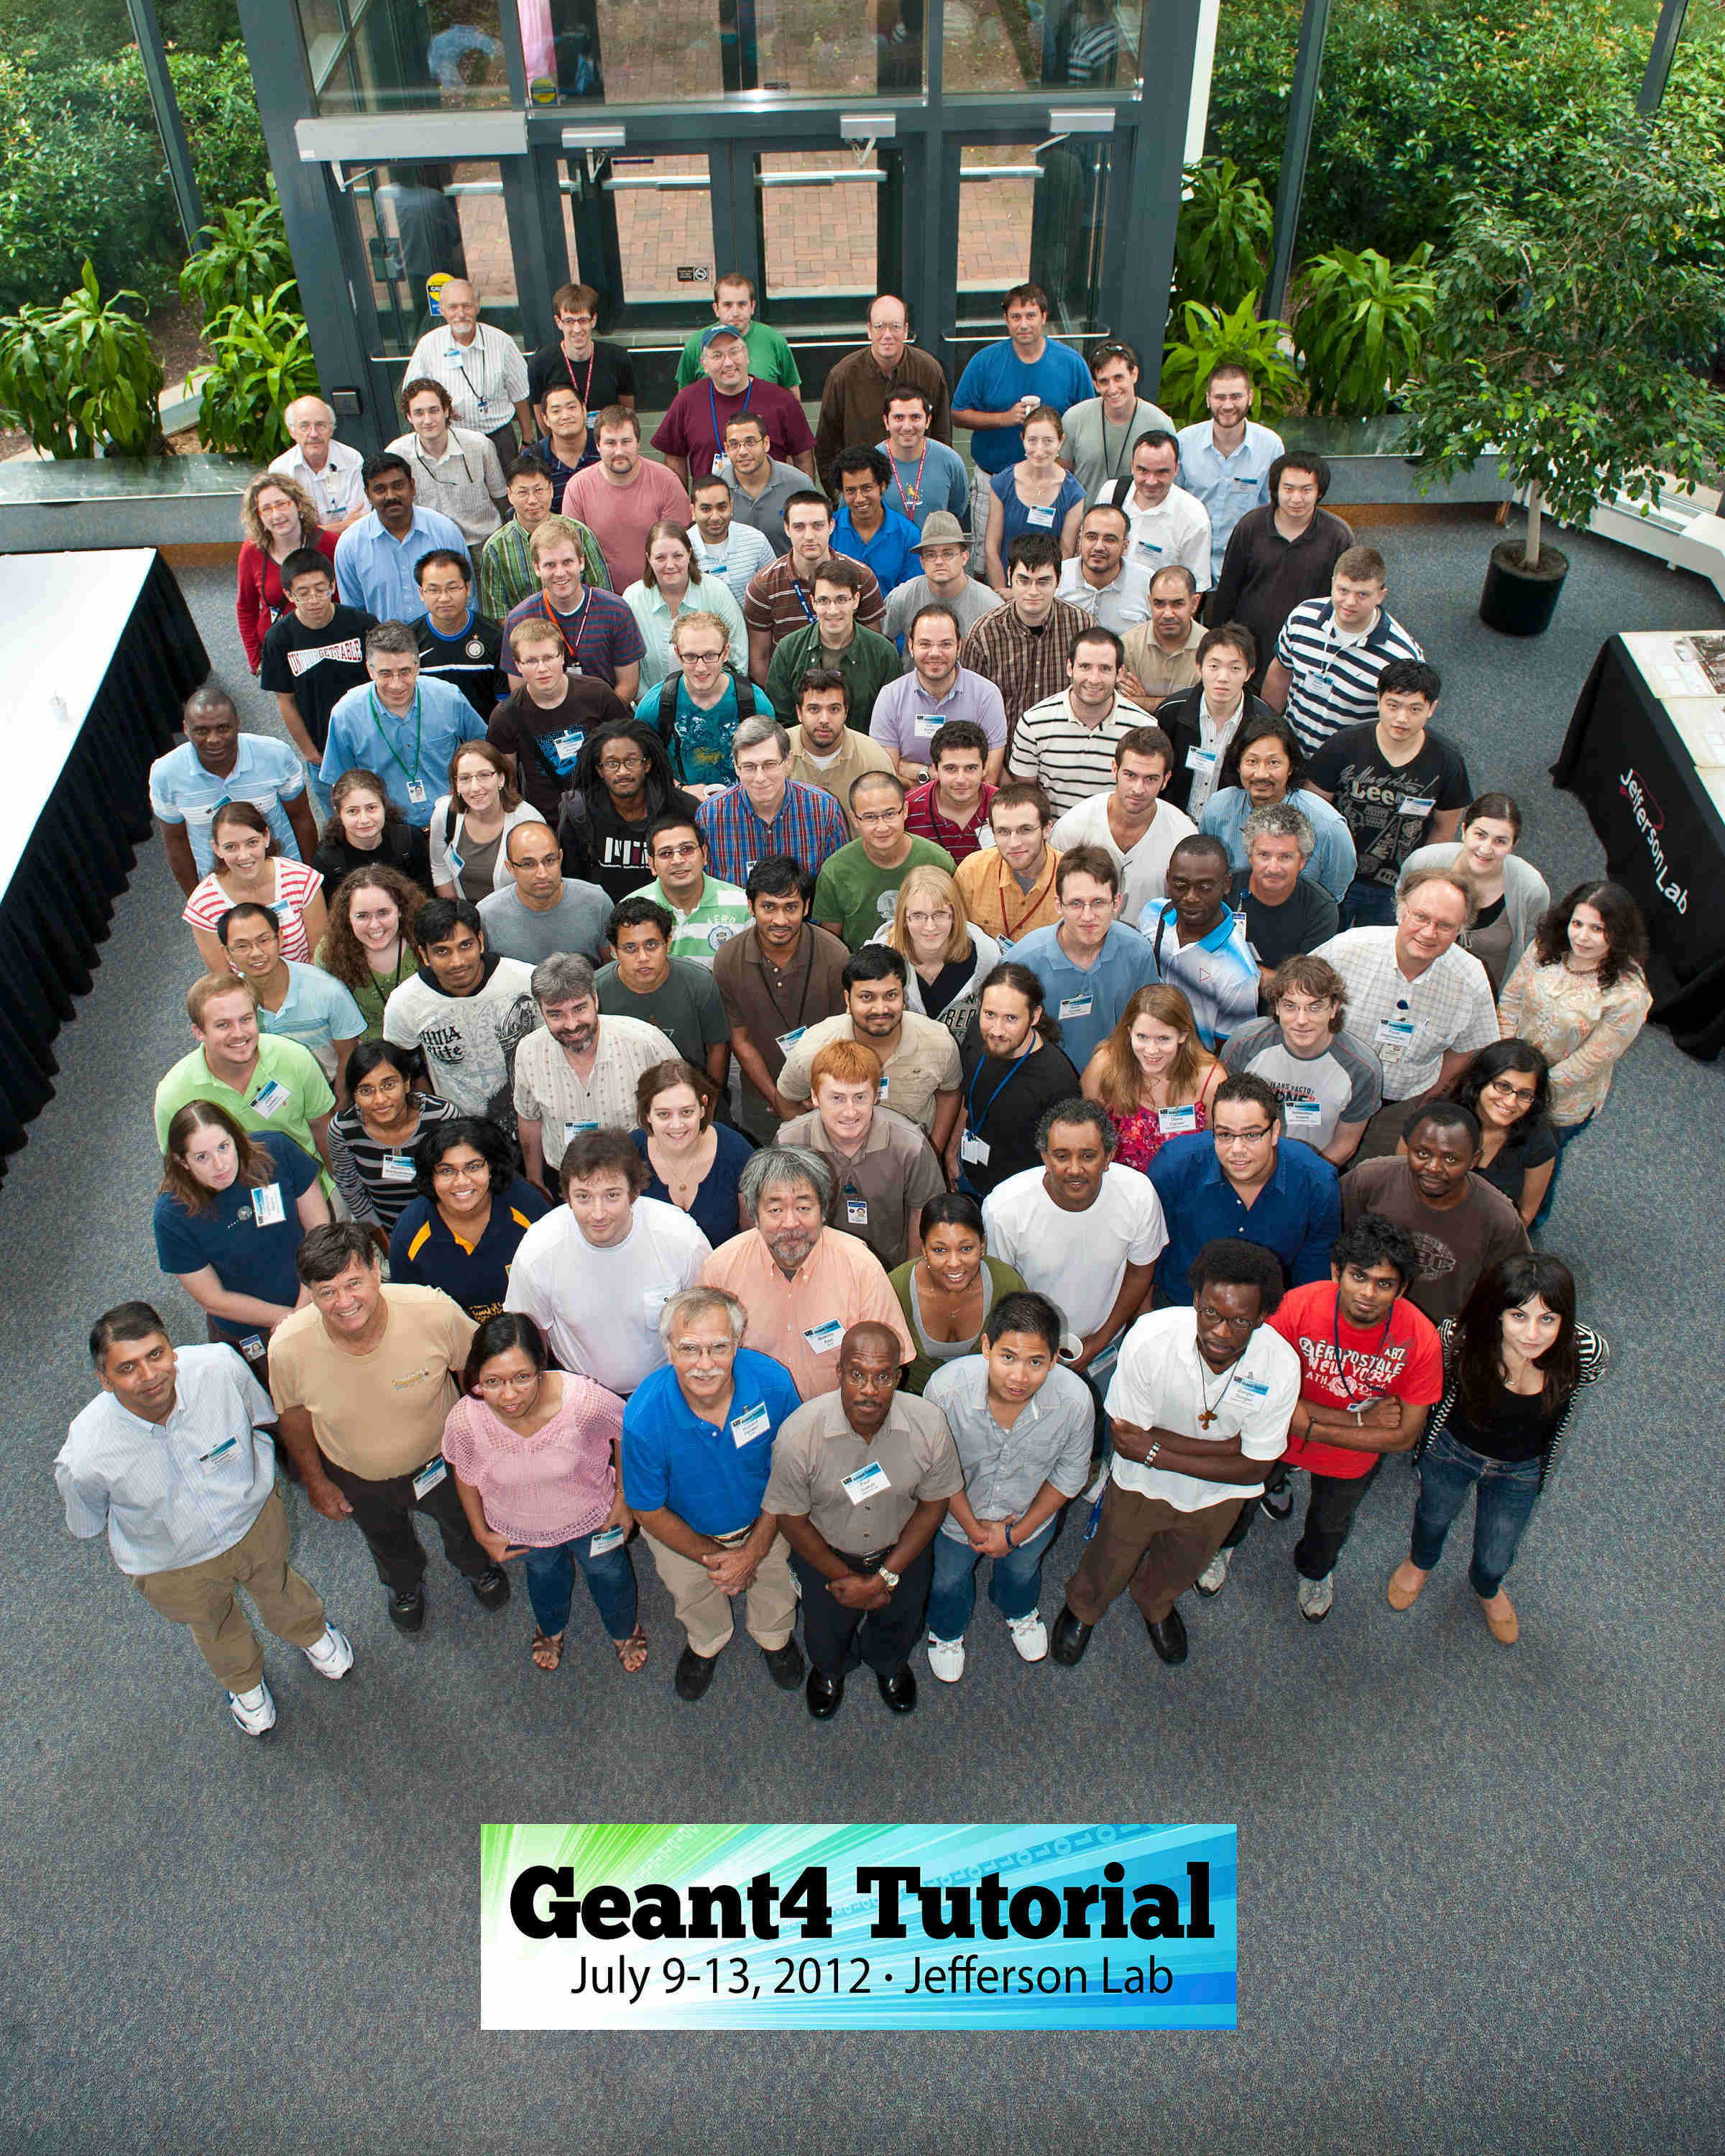
\includegraphics[width=\textwidth]{group8x10_lowres.jpg}
\end{columns}

}

\f{
\ft{Scientific Computing Survey}

\bi
\I Sponsored by User Group Board of Directors
\I Running Period: 4 weeks, starting July 23 through August 20, 2012
\I Questions: 16 multiple choice questions, 2 essay-type questions
\I Number of responses: 118
\I Impressions from written responses
    \bi
    \I standard package support desired (ROOT, GEANT) 
    \I large-scale data transfer on/off-site difficult
    \ei
\ei
}

\f{
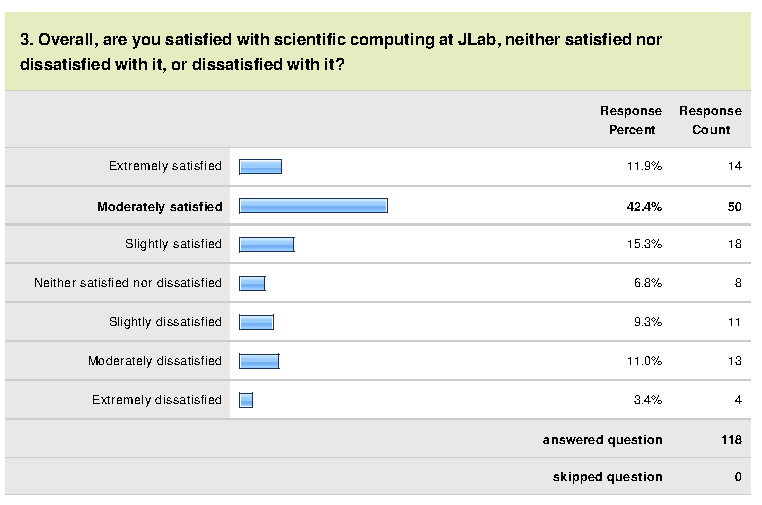
\includegraphics[width=4.5in]{q3.png}
}

\end{document}
